%
% Poster latex file for ADASS 2018
% Pey Lian Lim (lim@stsci.edu)
% Eric R. Jeschke (eric@naoj.org)
%
% [top-level file]
\nonstopmode

\documentclass[]{article}
\usepackage{graphicx}
% where can I find the graphics that will be imported for this version
\graphicspath{{./figures/}}

% Using \fbox you can draw a nice razor-thin border around images
\setlength\fboxsep{0pt}
\setlength\fboxrule{0.5pt}

% in case you want to embed any hyperlinks
%\usepackage{hyperref}

% for + and - signs in setting width etc
\usepackage{calc}

% scalable fonts
\usepackage[quiet]{fontspec}
\setmainfont[Mapping=tex-text,Scale=2.1]{DejaVu Serif}
\setsansfont[Mapping=tex-text,Scale=2.1]{DejaVu Sans}
\setmonofont[Mapping=tex-text,Scale=2.1]{DejaVu Sans Mono}
%\setmainfont[Mapping=tex-text,Scale=1.0]{Times New Roman}
%setsansfont[Mapping=tex-text,Scale=1.0]{Arial}
%setmonofont[Mapping=tex-text,Scale=1.0]{Courier New}

% for multiple columns
\usepackage{multicol}

% fancy boxes
\usepackage{fancybox}

% uncomment the actual desired size
%\def\mypaperwidth{33.11in} \def\mypaperheight{46.81in}    % A0
\def\mypaperwidth{27.83in} \def\mypaperheight{39.37in}     % B1
%\def\mypaperwidth{23.39in} \def\mypaperheight{33.1124in}  % A1
%\def\mypaperwidth{8.27in} \def\mypaperheight{11.69in}  % A4
\def\imgwd{6.0in}  % define image widths
% margin around edge of page
\def\mymargin{1in}

%% \def\mypaperwidth{11in} \def\mypaperheight{17.0in}     % Tabloid
%% \def\imgwd{2.5in}  % define image widths
%% \def\mymargin{0.25in}

% painful TeX calculation of 2*margin
\dimen87=\mymargin
\multiply\dimen87 by 2
\def\mydblmargin{\dimen87}

\usepackage[paperwidth=\mypaperwidth, paperheight=\mypaperheight,
            % margins are calculated from the trim + no print area
            top=\mymargin, bottom=\mymargin,
            left=\mymargin, right=\mymargin]{geometry}

\begin{document}

% dimensions of main writing area of page
\setlength{\textwidth}{\mypaperwidth-\mydblmargin}
%\setlength{\textwidth}{13in}
\setlength{\textheight}{\mypaperheight-\mydblmargin}

% TeX defines the content to begin at 1in offset from the side and
% top of the document (seemingly somewhat independent of margin
% settings).  These specify offsets to be added to the 1in defaults.
% You can calculate these or just tweak them until you get the result
% that you like.
\setlength{\hoffset}{-1.0in}
\setlength{\voffset}{-1.0in}

% width of margin notes area
\setlength{\marginparwidth}{0in}
% distance between margin and paragraph
\setlength{\marginparsep}{0in}

% footer configuration
\setlength{\footskip}{1em}

% header configuration
\setlength\headheight{0in}
\setlength\headsep{1em}

% margin tweaking
\setlength{\topmargin}{0.0in}
\setlength{\oddsidemargin}{1in}
% LEFT margin on even pages
\setlength{\evensidemargin}{1in}

% define explicitly set paragraph spacing
\newcommand{\para}{\vspace*{1em}}

\title{{\tt stginga}: Ginga Plugins for Data Analysis and Quality Assurance of
            HST and JWST Science Data}
\author{P. L. Lim (STScI) and E. R. Jeschke (NAOJ)}

% paragraph indentations
\setlength{\parindent}{0in}
% amount of space before each new paragraph begins
\setlength{\parskip}{0pt}

% comment to force even justification
\raggedright

%\begin{document}

\pagestyle{empty}

% interior facing page for book version
\begin{minipage}[t]{0.8\linewidth}
  \vspace{0pt}
\begin{center}
{\huge {\tt stginga}: Ginga Plugins for Data Analysis and Quality Assurance of
            HST and JWST Science Data }\\

\vspace*{1.5em}
Pey Lian Lim ({\tt lim@stsci.edu}),
Space Telescope Science Institute \\
Eric R. Jeschke ({\tt eric@naoj.org}),
National Astronomical Observatory of Japan
\end{center}
\end{minipage}
\hfill
\begin{minipage}[t]{0.15\linewidth}
  \vspace{0pt}
  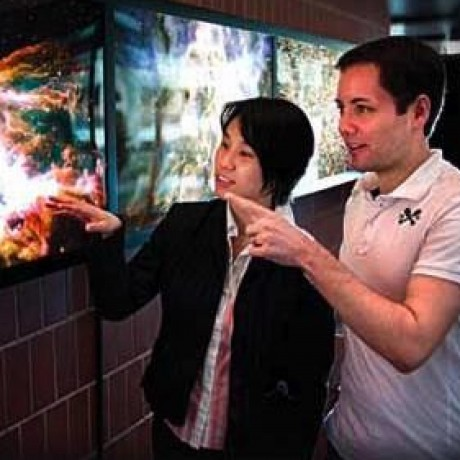
\includegraphics[width=2in]{pllim} \\
  {P. L. Lim}
\end{minipage}
%\vspace*{0in}
\vspace*{2em}

\noindent\hrulefill

\raggedcolumns
\setlength{\columnseprule}{1pt}
\setlength{\columnsep}{2em}

\medskip
\begin{multicols}{3}

\section*{Abstract}
{\tt stginga}\cite{stginga} is an image visualization package to assist
in data analysis and quality assurance of science data from Hubble Space
Telescope (HST) and James Webb Space Telescope (JWST).  It is based on the
Ginga\cite{ginga} toolkit for building scientific viewers.
In this poster, we will describe the main plugins developed for data
analysis and quality assurance tasks with {\tt stginga}.  We also discuss the
basic outline of writing a Ginga plugin, with pointers to documentation
and examples.

\section*{Introduction}

\begin{center}
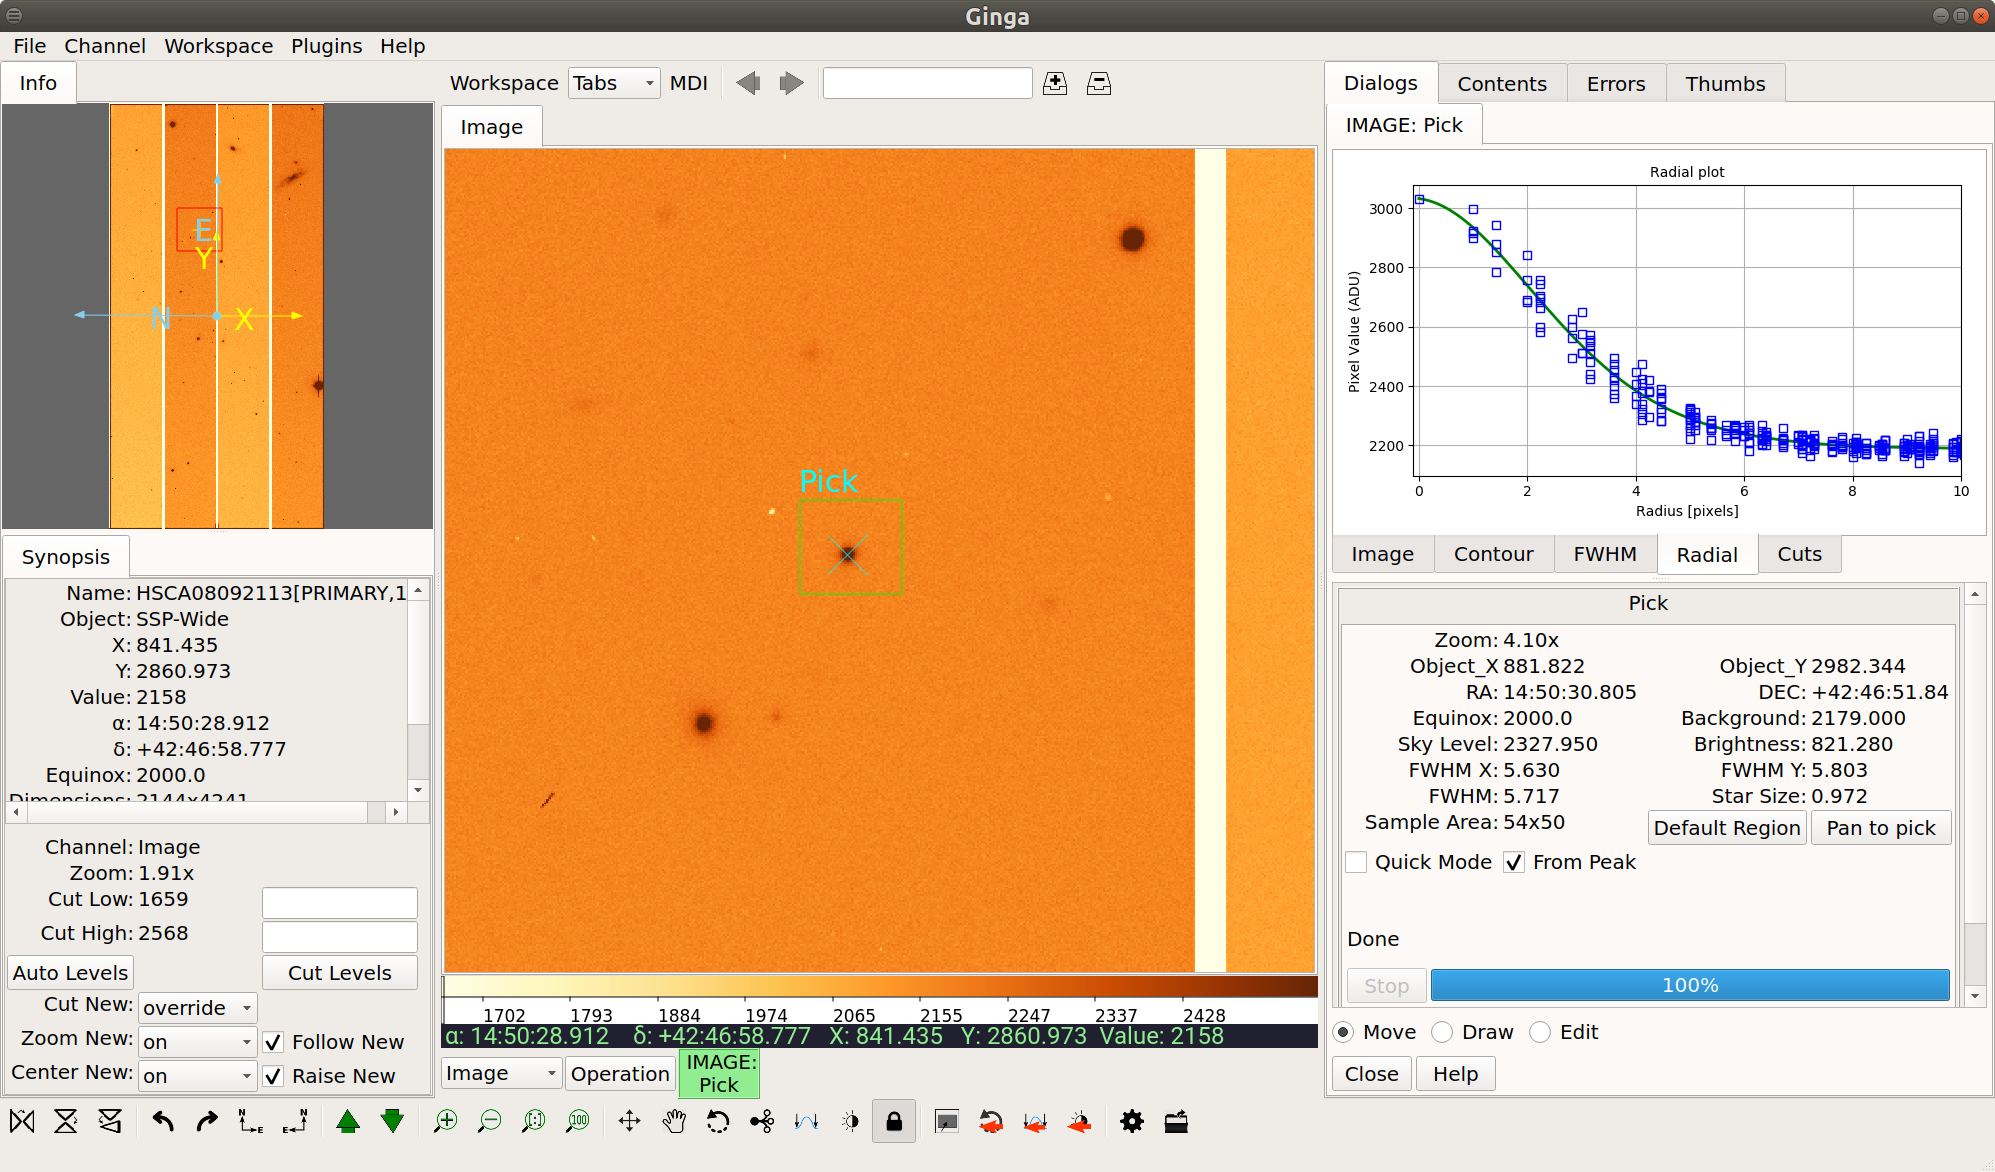
\includegraphics[width=8in]{ref_viewer}
\label{fig:refviewer}
\vspace*{0.4em}
{\small\em Figure 1: The Ginga reference viewer.}
\end{center}

\para
Ginga\cite{Jeschke15A} is a Python package that
implements a toolkit for building scientific viewers.  It provides
a \emph{reference viewer} (see Fig. 1), which features
a plugin architecture in which nearly every graphical feature of the
program is implemented by a Python plugin.
By implementing some new plugins for the HST and JWST data analysis and
quality assurance tasks, and combining these with a curated selection of
the distributed ``stock'' plugins, we were able to fairly quickly
develop a tool for use in the HST and JWST community.

\para
Ginga plugins are separated into global and local ones. A global plugin applies
to all images across all channels; thus, only once instance can be opened
in the whole Ginga session.
Meanwhile, a local plugin is associated with the channel it is started from;
therefore, one instance can be opened per channel and different instances
can be configured separately in the same Ginga session.
Plugins are currently not available when Ginga is used as part of Jupyter
Notebook/Lab. However, they are usable in a limited way via Ginga's remote
control (RC) interface, which will not be covered here.

\para
Currently, all the plugins are available in {\tt stginga} are local plugins.
Some plugins currently in Ginga originated from {\tt stginga}
(e.g., {\em ChangeHistory}, {\em SaveImage}, {\em TVMark}, and {\em TVMask})
when they were identified to be useful in general beyond HST or JWST.
All the screenshots shown in this poster used Qt5 backend, although they should
also work in Qt4, GTK 2, and GTK 3.

\section*{BackgroundSub}

\para
\begin{center}
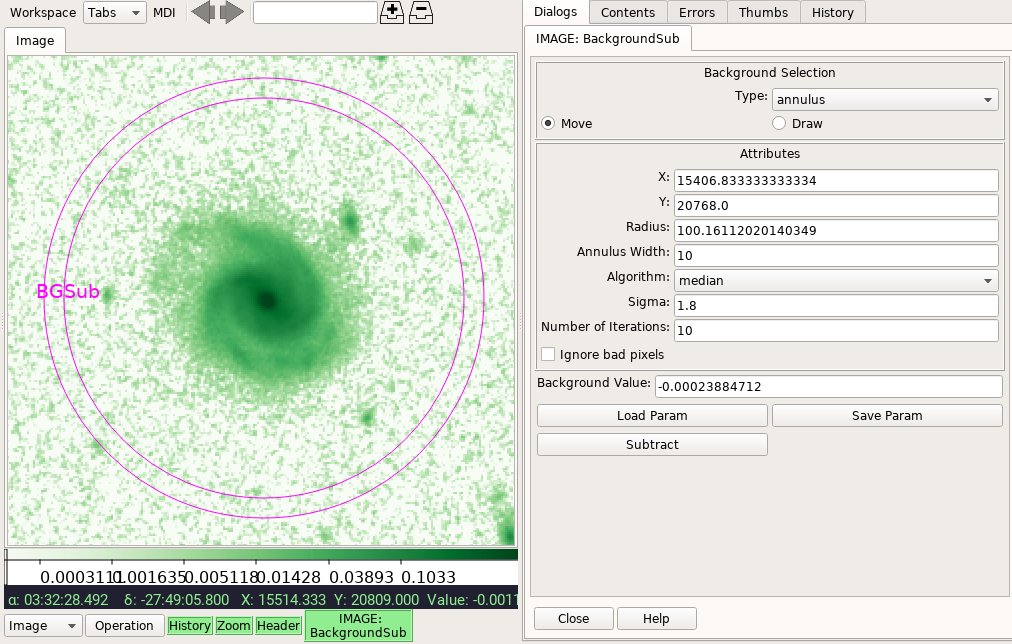
\includegraphics[width=8in]{plugin_backgroundsub} \\
\vspace*{0.4em}
\label{fig:plugin_backgroundsub}
{\small\em Figure 2: BackgroundSub plugin for background subtraction.}
\end{center}

\para
Curabitur vitae diam non enim vestibulum interdum. Duis ante orci,
molestie vitae vehicula venenatis, tincidunt ac pede. Neque porro
quisquam est, qui dolorem ipsum quia dolor sit amet, consectetur,
adipisci velit, sed quia non numquam eius modi tempora incidunt ut
labore et dolore magnam aliquam quaerat voluptatem. Ut enim ad minim
veniam, quis nostrud exercitation ullamco laboris nisi ut aliquip ex ea
commodo consequat. Phasellus faucibus molestie nisl. Integer in
sapien. Quisque porta. Aenean placerat. Mauris dictum facilisis
augue. Duis pulvinar. Nemo enim ipsam voluptatem quia voluptas sit
aspernatur aut odit aut fugit, sed quia consequuntur magni dolores eos
qui ratione voluptatem sequi nesciunt.

\section*{BadPixCorr}

\para
\begin{center}
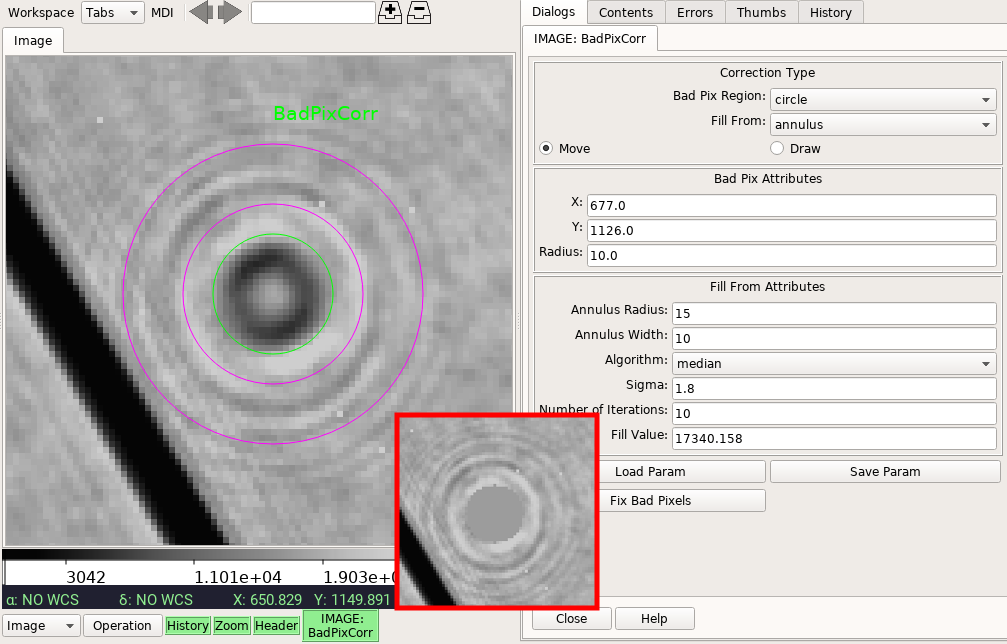
\includegraphics[width=8in]{plugin_badpixcorr.png}
\label{fig:plugin_badpixcorr}
\vspace*{0.4em}
{\small\em Figure 3: BadPixCorr plugin for bad pixel correction.}
\end{center}

\para
Etiam posuere lacus quis dolor. Pellentesque pretium lectus id
turpis. Etiam neque. Aliquam in lorem sit amet leo accumsan
lacinia. Duis viverra diam non justo. In rutrum. Curabitur bibendum
justo non orci. Neque porro quisquam est, qui dolorem ipsum quia dolor
sit amet, consectetur, adipisci velit, sed quia non numquam eius modi
tempora incidunt ut labore et dolore magnam aliquam quaerat
voluptatem. Maecenas sollicitudin. Vestibulum erat nulla, ullamcorper
nec, rutrum non, nonummy ac, erat. Nam quis nulla. Fusce suscipit libero
eget elit. Nullam justo enim, consectetuer nec, ullamcorper ac,
vestibulum in, elit. Integer malesuada. Cum sociis natoque penatibus et
magnis dis parturient montes, nascetur ridiculus mus. Donec vitae
arcu. Aliquam erat volutpat. Praesent id justo in neque elementum
ultrices. Nam sed tellus id magna elementum tincidunt. Nullam lectus
justo, vulputate eget mollis sed, tempor sed magna.

\para
Proin in tellus sit amet nibh dignissim sagittis. Curabitur bibendum
justo non orci. Nulla non lectus sed nisl molestie malesuada. In
rutrum. Class aptent taciti sociosqu ad litora torquent per conubia
nostra, per inceptos hymenaeos. Nullam at arcu a est sollicitudin
euismod. Quisque tincidunt scelerisque libero. Nullam eget nisl. Cras
pede libero, dapibus nec, pretium sit amet, tempor quis. Maecenas
libero. Curabitur sagittis hendrerit ante. Phasellus rhoncus. Sed
convallis magna eu sem. Integer lacinia.

\section*{DQInspect}

\para
\begin{center}
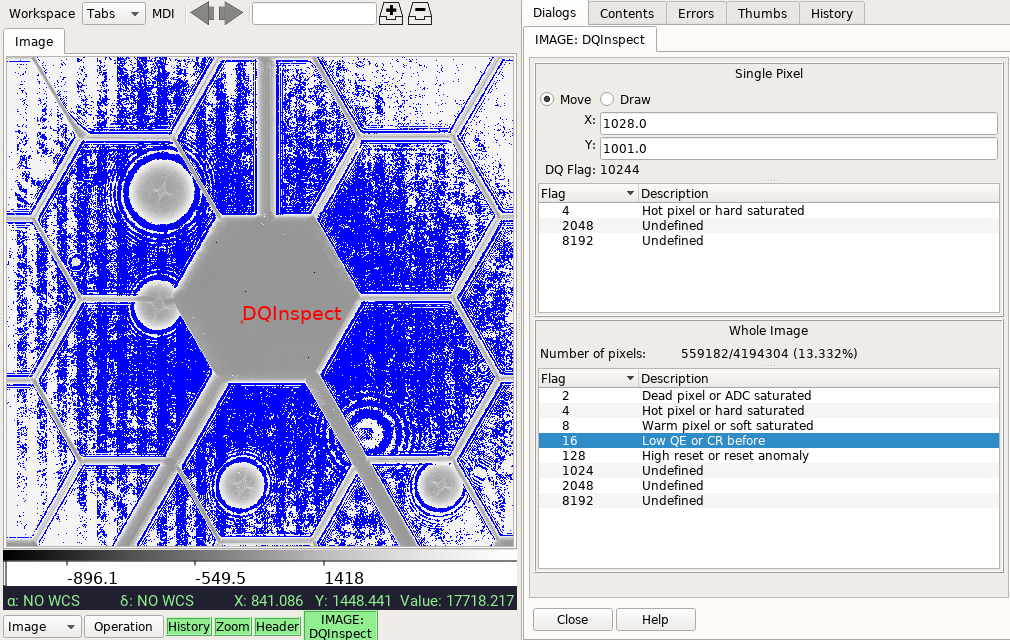
\includegraphics[width=8in]{plugin_dqinspect} \\
\vspace*{0.4em}
\label{fig:plugin_dqinspect}
{\small\em Figure 4: DQInspect plugin for data quality inspection.}
\end{center}

\para
In enim a arcu imperdiet malesuada. Nulla non arcu lacinia neque
faucibus fringilla. In dapibus augue non sapien. Fusce consectetuer
risus a nunc. Nullam sapien sem, ornare ac, nonummy non, lobortis a
enim. Sed elit dui, pellentesque a, faucibus vel, interdum nec,
diam. Aliquam id dolor. Nam sed tellus id magna elementum
tincidunt. Phasellus et lorem id felis nonummy placerat. Nulla accumsan,
elit sit amet varius semper, nulla mauris mollis quam, tempor suscipit
diam nulla vel leo. Nunc dapibus tortor vel mi dapibus
sollicitudin. Quisque porta. Praesent vitae arcu tempor neque lacinia
pretium.

\section*{SNRCalc}

\para
\begin{center}
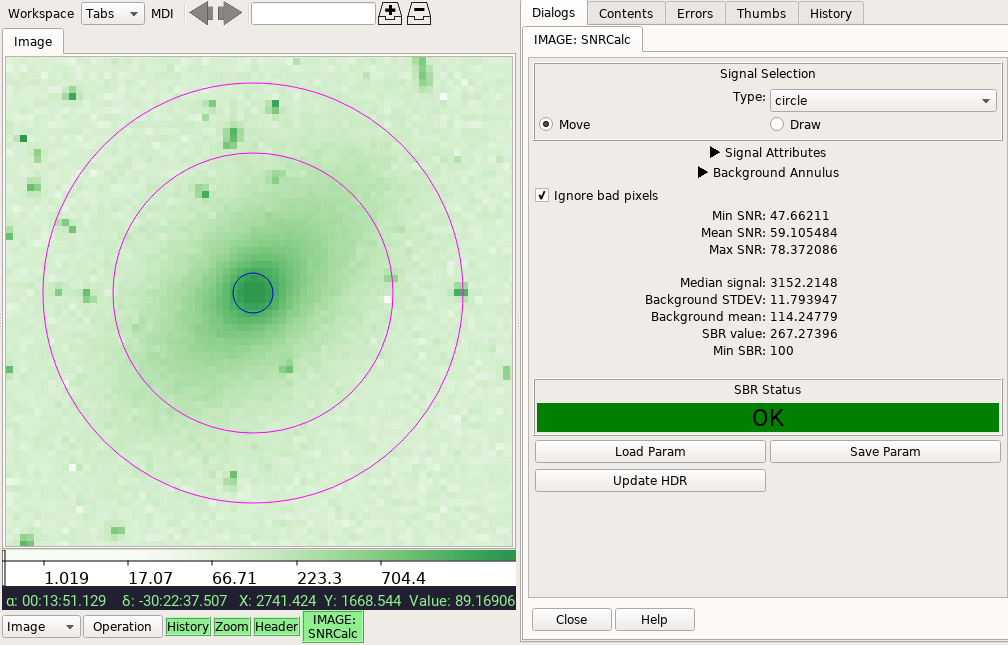
\includegraphics[width=8in]{plugin_snrcalc} \\
\vspace*{0.4em}
\label{fig:plugin_snrcalc}
{\small\em Figure 5: SNRCalc plugin for SNR calculation.}
\end{center}

\para
Etiam ligula pede, sagittis quis, interdum ultricies, scelerisque
eu. Sed convallis magna eu sem. Integer pellentesque quam vel
velit. Pellentesque ipsum. Pellentesque arcu. Ut enim ad minima veniam,
quis nostrum exercitationem ullam corporis suscipit laboriosam, nisi ut
aliquid ex ea commodi consequatur? Temporibus autem quibusdam et aut
officiis debitis aut rerum necessitatibus saepe eveniet ut et voluptates
repudiandae sint et molestiae non recusandae. Proin in tellus sit amet
nibh dignissim sagittis. Etiam posuere lacus quis dolor. Integer
lacinia. Aenean placerat. Maecenas libero. Ut tempus purus at
lorem. Phasellus faucibus molestie nisl. Fusce consectetuer risus a
nunc. Nullam faucibus mi quis velit. Duis condimentum augue id magna
semper rutrum.

\section*{Writing a Ginga plugin}

\para
Pellentesque habitant morbi tristique senectus et netus et malesuada
fames ac turpis egestas. Duis pulvinar. Fusce nibh. Suspendisse
nisl. Sed vel lectus. Donec odio tempus molestie, porttitor ut, iaculis
quis, sem. Etiam dictum tincidunt diam. Pellentesque sapien. Etiam
commodo dui eget wisi. Nemo enim ipsam voluptatem quia voluptas sit
aspernatur aut odit aut fugit, sed quia consequuntur magni dolores eos
qui ratione voluptatem sequi nesciunt. Proin in tellus sit amet nibh
dignissim sagittis. Aliquam in lorem sit amet leo accumsan
lacinia. Nullam faucibus mi quis velit. Sed ut perspiciatis unde omnis
iste natus error sit voluptatem accusantium doloremque laudantium, totam
rem aperiam, eaque ipsa quae ab illo inventore veritatis et quasi
architecto beatae vitae dicta sunt explicabo. Nullam sapien sem, ornare
ac, nonummy non, lobortis a enim. Etiam bibendum elit eget erat. Nunc
tincidunt ante vitae massa.

\para
Curabitur ligula sapien, pulvinar a vestibulum quis, facilisis vel
sapien. Suspendisse nisl. Curabitur sagittis hendrerit ante. Mauris
tincidunt sem sed arcu. Pellentesque arcu. Aenean placerat. Neque porro
quisquam est, qui dolorem ipsum quia dolor sit amet, consectetur,
adipisci velit, sed quia non numquam eius modi tempora incidunt ut
labore et dolore magnam aliquam quaerat voluptatem. Itaque earum rerum
hic tenetur a sapiente delectus, ut aut reiciendis voluptatibus maiores
alias consequatur aut perferendis doloribus asperiores repellat. In
laoreet, magna id viverra tincidunt, sem odio bibendum justo, vel
imperdiet sapien wisi sed libero. Fusce dui leo, imperdiet in, aliquam
sit amet, feugiat eu, orci. Aliquam erat volutpat. Fusce tellus odio,
dapibus id fermentum quis, suscipit id erat. Aliquam ante. Vivamus ac
leo pretium faucibus. Etiam posuere lacus quis dolor. Nullam dapibus
fermentum ipsum. Praesent dapibus.

%% \para
%% Duis aute irure dolor in reprehenderit in voluptate velit esse cillum
%% dolore eu fugiat nulla pariatur. Donec ipsum massa, ullamcorper in,
%% auctor et, scelerisque sed, est. Proin in tellus sit amet nibh dignissim
%% sagittis. Fusce tellus. Sed ac dolor sit amet purus malesuada
%% congue. Aliquam erat volutpat. Pellentesque habitant morbi tristique
%% senectus et netus et malesuada fames ac turpis egestas. Etiam egestas
%% wisi a erat. Nullam lectus justo, vulputate eget mollis sed, tempor sed
%% magna. Pellentesque arcu. Cum sociis natoque penatibus et magnis dis
%% parturient montes, nascetur ridiculus mus. Maecenas lorem. Maecenas
%% libero.

\para
Fusce consectetuer risus a nunc. Etiam posuere lacus quis dolor. Nullam
feugiat, turpis at pulvinar vulputate, erat libero tristique tellus, nec
bibendum odio risus sit amet ante. Etiam commodo dui eget wisi. Duis
bibendum, lectus ut viverra rhoncus, dolor nunc faucibus libero, eget
facilisis enim ipsum id lacus. Mauris elementum mauris vitae
tortor. Duis pulvinar. Etiam neque. Mauris metus. Duis sapien nunc,
commodo et, interdum suscipit, sollicitudin et, dolor. Sed convallis
magna eu sem. Etiam ligula pede, sagittis quis, interdum ultricies,
scelerisque eu. Nulla non arcu lacinia neque faucibus fringilla. Duis
aute irure dolor in reprehenderit in voluptate velit esse cillum dolore
eu fugiat nulla pariatur. Mauris metus. Etiam bibendum elit eget
erat. Phasellus enim erat, vestibulum vel, aliquam a, posuere eu,
velit. Fusce dui leo, imperdiet in, aliquam sit amet, feugiat eu,
orci. Mauris dictum facilisis augue. Vivamus luctus egestas leo.

\section*{Conclusion}

{\tt stginga} utilizes Ginga plugins to support HST and JWST data analysis,
which includes background subtraction, bad pixel correction, data quality flags
inspection, and signal-to-noise calculations.

\para
Writing Ginga plugins can be an expedient way to develop graphical data
analysis and quality assurance tasks, by leveraging the combination of
Python, a lean Ginga plugin API, and the burgeoning number of open-source
astronomical Python modules.

\para
Both {\tt stginga} and {\tt ginga} are installable via {\tt pip}. Alternately,
if you use {\tt conda}, they are also available on AstroConda\cite{astroconda},
in addition to {\tt ginga} being in  {\tt conda-forge} too. Their development
versions could be cloned from GitHub. Both are open-source and licensed under
3-clause BSD.

\bibliographystyle{abbrv}
\bibliography{poster}

\end{multicols}

\end{document}
